\chapter{Optimization of DSFDM/FFWI code in shared node, MESCA II}
\section{DSFDM/FFWI}
\subsection{Description}
The DSFDM/FFWI is a package which contains parallel computer codes to perform seismic modeling and fullwaveform inversion in the frequency domain. These codes have have been designed to execute modeling/inversion in 1, 2, 3 dimension media. According to the authors, only the 3D version is tested and Documented [doc DSfDm]. The DSFDM code is the seismic modeling code, while the FFWI code performs the inversion, using most of the subroutines implemented in DSFDM.Moreover,the DSFDM/FFWI codes assume visco-acoustic submarine supports in which vertical transverse isotropy can be taken into account.

Seismic modeling is performed in the frequency domain with a finite-difference method on a uniform Cartesian grid ([Operto et al., 2007][Brossier et al., 2010]; [Operto et al., 2014]). The linear system resulting from
the discretization of the time-harmonic wave equation is solved with a sparse direct solver. Sources and receivers, which can be processed in a reciprocal way, can be considered at arbitrary positions in coarse finite-difference grids with the sinc parameterization developed by Hicks (Hicks, 2002). Absorbing boundary conditions are perfectly-matched layers (PMLs) ([B\'{e}renger, 1994]; [Operto et al., 2007]). A free-surface boundary condition can be used along arbitrary tomography by forcing the pressure wave-field to 0 along this boundary. All of the tasks performed during seismic modeling (building impedance matrix, building right-hand side vectors, call of MUMPS subroutines, writing of solutions and extraction at receiver solutions) are implemented in the DSFDM code.

FFWI code is implemented with various local optimization methods. Recorded data are provided in the frequency-domain using an adaptation of the Seismic Unix (SU) format. The data are complex-valued (in single precision) and the frequency interval is uniform. The first frequency, the number of frequency and the frequency interval must be provided at specific locations in the SU headers. The numerical optimization is performed with the SEISCOPE optimization toolbox and allows for steepest-descent, conjugate gradient,l-BFGS and truncated Newton optimizations ([M\'{e}tivier and Brossier, 2016]). Seismic modeling and inversion are performed on the same Cartesian grid. Source wavelet estimation can be performed at each iteration of the FWI. Only the preconditioned steepest-descent optimization was tested, although conjugate gradient and l-BFGS optimizations are interfaced with the FFWI code. Interfacing Gauss-Newton and Newton truncated optimizations is the aim of ongoing work. The code has been tested for the update of the vertical wavespeed only. An application to real data is shown in [Operto et al., 2015]. Multi-parameter gradients are implemented but still need to be validated.

\section{MUMPS Solver}
MUMPS ("MUltifrontal Massively Parallel Solver") is a package for solving systems of linear equations of the form $ Ax = b$, where $ A $ is a square sparse matrix that can be either unsymmetric, symmetric positive definite, or general symmetric, on distributed memory computers. The MUMPS package is designed to solve linear equations by using a direct method based on a multifrontal approach which performs a Gaussian factorization
$$ A = LU $$ 
where $ L $ is a lower triangular matrix and $ U $ an upper triangular matrix. If the matrix is symmetric then
the factorization
$$ A = LDL^{T}$$
where D is block diagonal matrix with blocks of order 1 or 2 on the diagonal is performed. 

MUMPS solvers the result of collaboration between different partners working in the MUMPS project since 1996. Todays, the MUMPS team include CERFACS, CNRS, ENS-Lyon, INRIA, INPT, University of Bordeaux. In the recent years, the popularity of MUMPS package has increased in different countries and different scientific projects. It has known different version during the years with real improvement of the LU factorization methods. The recent research of MUMPS project is focused on the Block-Low rank option that allows decreasing the complexity of sparse direct solvers on problems arising from partial differential equations is provided for experimentation purpose. 

A matrix A of size $ m \times n $ is said to be low rank if it can be approximated by a low-rank product $ \tilde{A} = XY^{T}$ of rank $ k_{\epsilon} $, such that $ k_{\epsilon}(m+n)\leq mn $ and $ \Vert \tilde{A} - A \Vert \leq  k_{\epsilon} $. The first condition states that the low-rank form of the matrix requires less storage than the standard form, whereas the second condition simply states that the approximation is of good enough accuracy. Using the low-rank form also allows for a reduction of the number of floating-point operations performed in many kernels (e.g., matrix-matrix multiplication).

Thanks to the low-rank compression, the theoretical complexity of the factorization is reduced from $ O(n^{6})$ to $ O(n^{5.5})$ and can be further reduced to $ O(n^{5} \log 5 )$ with the best variant of the BLR format ([Amestoy et al., 2016b]).

\section{Tools}
As we mentioned above, this DSFDM/FFWI version use MUMPS package to solve the linear system of discretized wave propagation equation. We need to install different packages for MUMPS dependencies as well as DSFDM/FFWI. MUMPS can be installed in sequential version. In the same way, it can be used with multithreaded machine (with OpenMP) or with parallel version (distributed memory MPI based). We need these packages for MUMPS installation:
\begin{itemize}
\item \textbf{BLAS library}: BLAS (\textit{Basic Linear Algebra Subprograms}) are routines that provide standard building blocks for performing basic vector and matrix operations. The Level 1 BLAS perform scalar, vector and vector-vector operations, the Level 2 BLAS perform matrix-vector operations, and the Level 3 BLAS perform matrix-matrix operations. BLAS is written in Fortan and it has an optimized sequential or multithreaded version.
\item LAPACK library: LAPACK or Linear Algebra PACKage routines are written so that as much as possible of the computation is performed by calls to the Basic Linear Algebra Subprograms (BLAS). LAPACK is designed at the outset to exploit the Level 3 BLAS. Because of the coarse granularity of the Level 3 BLAS operations, their use promotes high efficiency on many high-performance computers, particularly if specially coded implementations are provided by the manufacturer.
\item ScaLAPACK library: Similar to LAPACK, ScaLAPACK is a library of high-performance linear algebra routines for parallel distributed memory machines. It solves dense and banded linear systems, least squares problems, eigenvalue problems, and singular value problems. The use of ScaLAPACK provides efficiency, scalability, reliability, portability, flexibility, and ease of use (by making the interface to LAPACK and ScaLAPACK look as similar as possible). 
\item BLACS library: In the context of distributed parallel machines, the BLACS (Basic Linear Algebra Communication Subprograms) routines is created to make easy linear algebra oriented message passing interface that may be implemented efficiently and uniformly across a large range of distributed memory platforms.
\item OpenMP library: As we discuss in the section \ref{openMP}, this package allows parallel programming in  shared memory multi-core platforms. The openMP directives improves strongly the performance of MUMPS. OpenMP parallel regions of MUMPS can be set through the OMP\_NUM\_THREADS environment variable. 
\item MPI library: 
\item Others
\end{itemize}

\section{Installation of DSFDM/FFWI}
\subsection{Description of nodes}
\section{Methodology}
In this study, our aim is to evaluate the capacity of the DSFDM/FFWI code to process large test cases on MESCA-II node and to improve the performance of the code in this architecture. This implies how to keep the code scalable when the memory consumption and MPI communications are increasing. In [], the authors show that the memory consumption and elapsed time are mostly based on LU matrix factorisation doing by MUMPS package. Their results explain in more details this fact [].  The MUMPS team has developed the BLR option to improve the performance of the storing of LU matrix values (Amestoy et al. []). 
As we discuss above (see \ref{optimization}), the optimization of DSFDM/FFWI can be seen in multiple levels. In this study, we will focus on scalability study (strongly and weakly) and different profiling methods to analyse the performance of the code.  
\section{Scalability study}
The scalability, as we discussed in section \ref{scalability}, is the coarse grained of the study of performance. It can be measured in two scales: strong scaling and weak scaling. Here, we study these two scales in different  nodes cluster such as Mesca and classical nodes. When we say classical nodes it refers the other nodes different to Mesca.  
\subsection{Strong Scalability}
This study allow us to understand how much faster our DSFDM/FFWI code is with N processors by fixing the size of the problem. Firstly, we perform different test cases in classical nodes to be comparing the performance with Mesca. To study the scalability, we use the homogeneous isotropic model that aims to validate DFSFDM against an analytical solution computed in an homogeneous infinite acoustic isotropic ($ianiso=0$) medium (Docffwi). According to the documentation, we fix, firstly, the size of the problem to be grid $(n1,n2,n3)=(41,41,121)$ ie. $ 4km \times 4km \times 12km$ (depth,X,Y). The others parameters are the same as the documentation. The wavespeed and the density are respectively equal to $ 1.5km/s $ and $ 1000km/m3 $. The grid interval is $ 100m$. The frequency is $3.72Hz$. The shot coordinates in meters are $ (x1, x2, x3) = (1000, 2000, 2000)$.

The results obtained in Figures \ref{cube_homogeneous_isotropic}-\ref{fig2_log_homogeneous_isotropic} show the comparison of \textbf{DSFDM} with the analytical solution (\textbf{FDTD}).
 
In the first test case, we run the code in a classical node such that the architecture is given in Table \ref{mannyNode} \newline

\begin{table}[!h]
\centering

\begin{tabular}{|l|l|}
\hline
Number of sockets (CPUs) & 2 sockets Intel(R) Xeon(R) CPU E5-2697 v2 	\\	
\hline
Number of Core(s) & 2 * 12 cores per socket at the nominal frequency 2.70GHz	\\	
\hline
Hyperthreading & activated			\\
\hline
Number of Thread(s) &  2 * 24 threads per cpu	\\
\hline
Shared Memory & 2*32 GB DDR*  (* unknown) \\	
\hline		
L1d/L1i cache &         32K	\\		
\hline
L2 cache &              256K	\\	
\hline	
L3 cache &             30720 KB	\\
\hline
\end{tabular}
\caption{Architecture of classical nodes}
\label{mannyNode}
\end{table}

The table \ref{manny} shows the computational resources used when the code is performing in this node.
\begin{table}[!h]
\centering

\begin{tabular}{lllllllll}
Grid dimensions & npml & \#u & \#n & \#MPI & \#th & $Mem_{LU}(Gb)$ & $T_{LU}(s)$ & $T(s)$ \\
 \hline
$41 \times 41 \times 121$ & 8 & 1 & 1 & 2  & 10 & 6,7 &  17.76 & 23.77 
\end{tabular}
\caption{Homogeneous Isotropic running on classical node: \#u($ 10^{6} $): number of unknowns. \#n: number of nodes. \#MPI: number of MPI process. \#th: number of threads per MPI process. $Mem_{LU}(Gb)$: Memory for LU
factorization in Gbytes. $T_{LU}(s)$: Elapsed time for factorization in s. $ T(s)$: Running time}
\label{manny}
\end{table}

Secondly, we execute the same test case with the same parameters in the Mesca node. The architecture of this node is showing in table \ref{mescaNode}.

\begin{table}[!h]
\centering
\begin{tabular}{|l|l|}
\hline
Number of sockets (CPUs) & 8 sockets Intel(R) Xeon(R) CPU E7-8890 v4 	\\	
\hline
Number of Core(s) & 8 * 24 cores cores at the nominal frequency 2.20GHz	\\	
\hline
Hyperthreading & deactivated			\\
\hline
Number of Thread(s) &  8 * 24 threads per cpu	\\
\hline
Shared Memory & 8*340 GB DDR*  (* unknown)   \\	
\hline		
L1d/L1i cache &         32K	\\		
\hline
L2 cache &              256K	\\	
\hline	
L3 cache &              61440K	\\
\hline
\end{tabular}
\caption{Architecture of Mesca II node}
\label{mescaNode}
\end{table}

These results are shown in the table \ref{Mesca1}

\begin{table}[!h]
\centering

\begin{tabular}{lllllllll}
Grid dimensions & npml & \#u & \#n & \#MPI & \#th & $Mem_{LU}(Gb)$ & $T_{LU}(s)$ & $T(s)$ \\
 \hline
$41 \times 41 \times 121$ & 8 & 1 & 1 & 2  & 10 & 6,7 &  17.73 & 25.048 
\end{tabular}
\caption{Homogeneous Isotropic running on Mesca II node}
\label{Mesca1}
\end{table}

By using two MPI processes and ten threads, the classical node shows almost the same performance as Mesca(
 $T_{LU}(s)\thickapprox 17.7 s$). In addition, the total memory allocated for factorization was  6.7 Gigabyte.The time of LU factorization takes 74 \% and 70 \% respectively in the classical node and Mesca. This type of node will be used for rest of the simulation. The results are shown in tables \ref{Mesca1} and \ref{manny}. \newline
\begin{figure}
\centering 
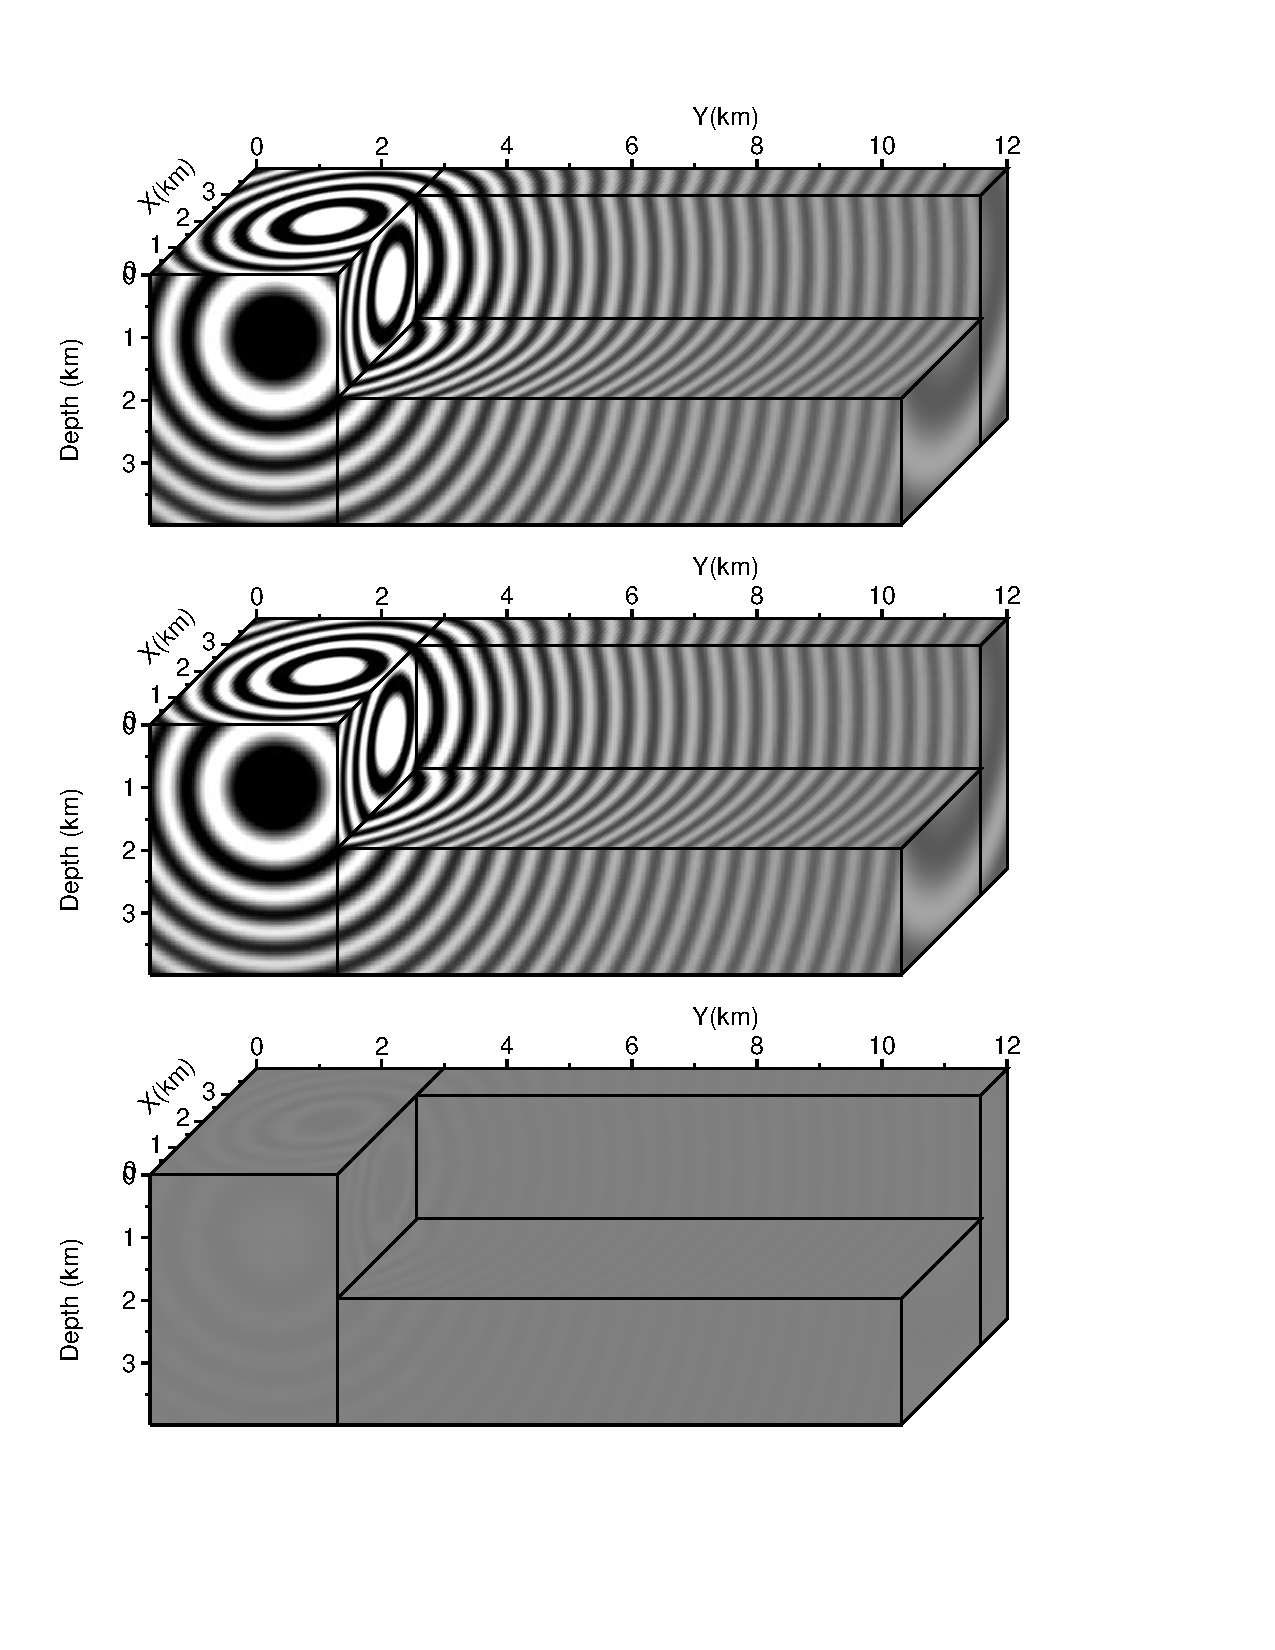
\includegraphics[width=0.7\textwidth]{images/fig_dsfdm/fig_cube_homogeneous_isotropic.pdf}
\caption{Homogeneous Isotropic. Infinite homogeneous isotropic medium. Validation against analytical
solution. a) DSFDM solution. b) Analytical solution. c) Difference.}
\label{cube_homogeneous_isotropic} 

\end{figure}
\begin{figure}[]
\centering 
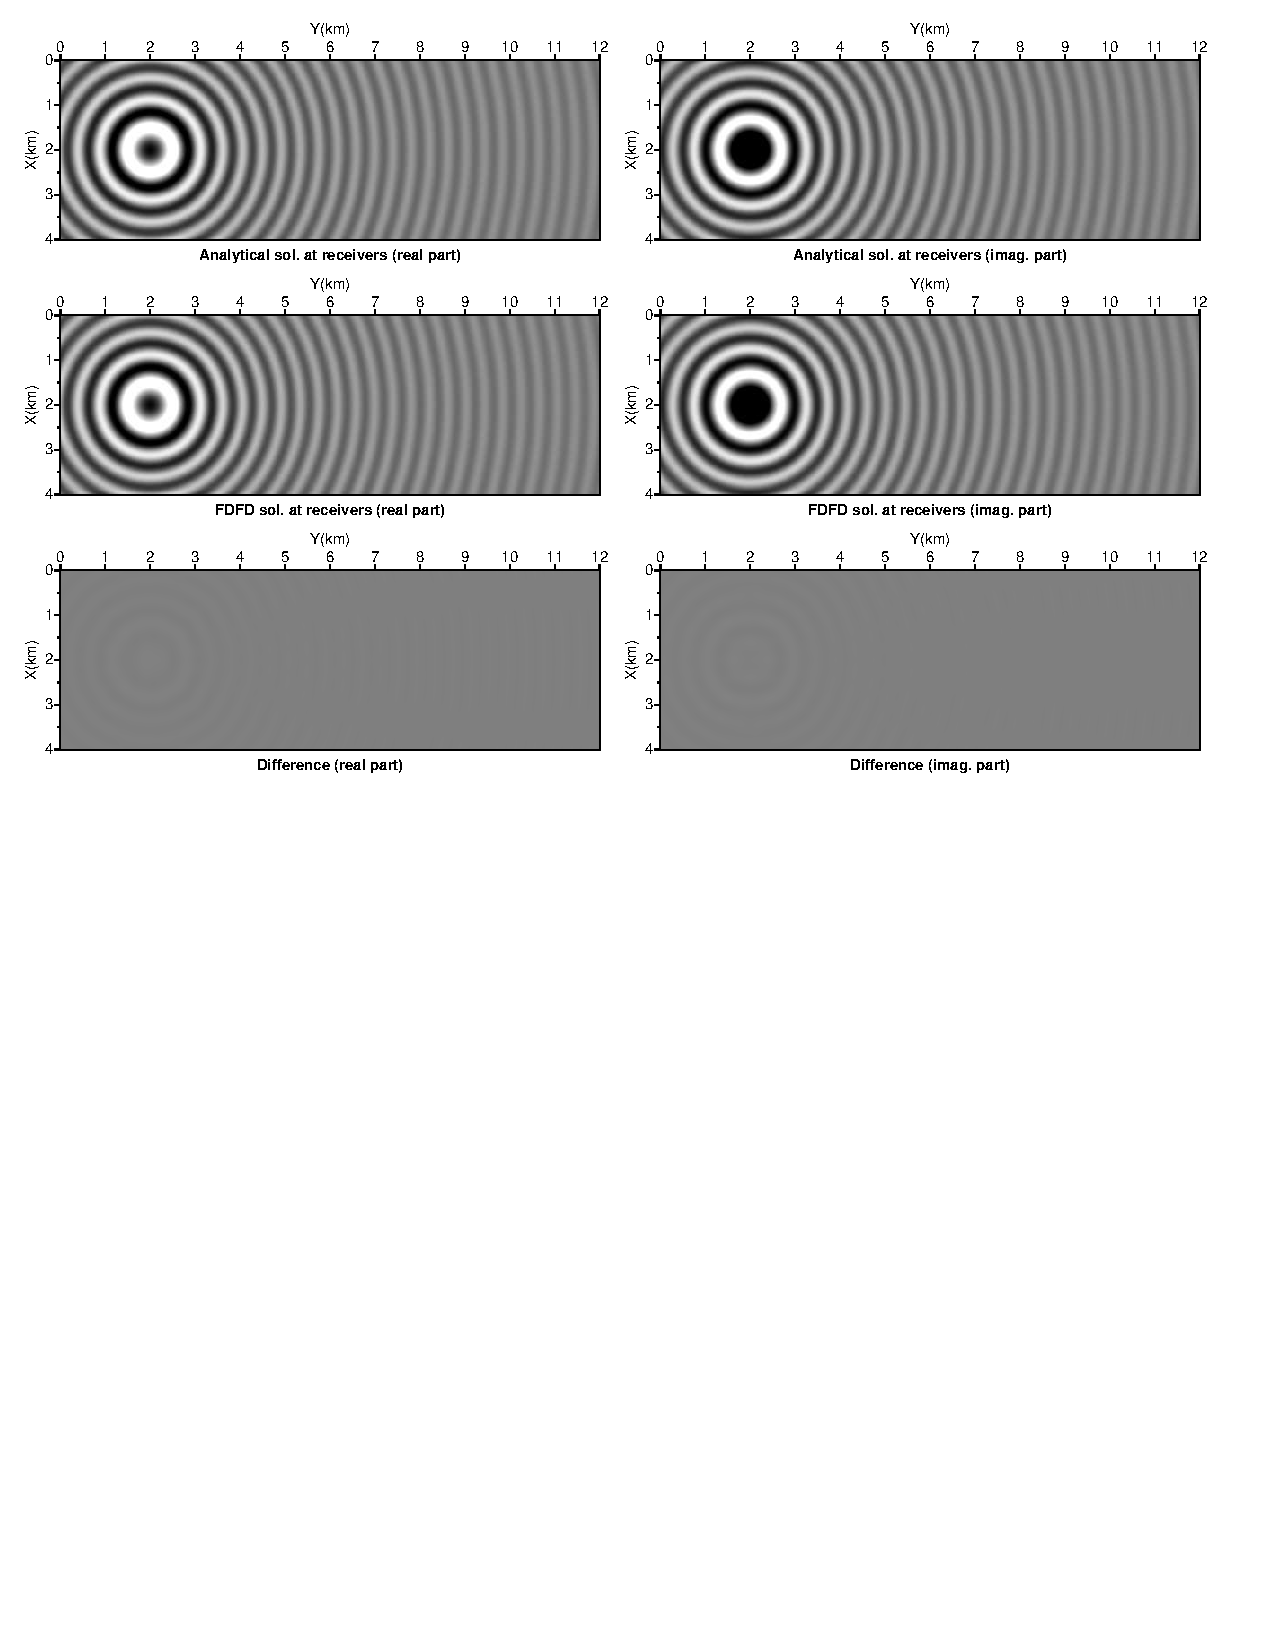
\includegraphics[width=0.7\textwidth]{images/fig_dsfdm/fig_rec_snap_homogeneous_isotropic.pdf}
\caption{Homogeneous Isotropic.  Infinite homogeneous isotropic medium. Validation against analytical
solution. Solution at receiver positions, 1km below the surface.}
\label{rec_snap_homogeneous_isotropic} 
\end{figure}
\begin{figure}[]
\centering 
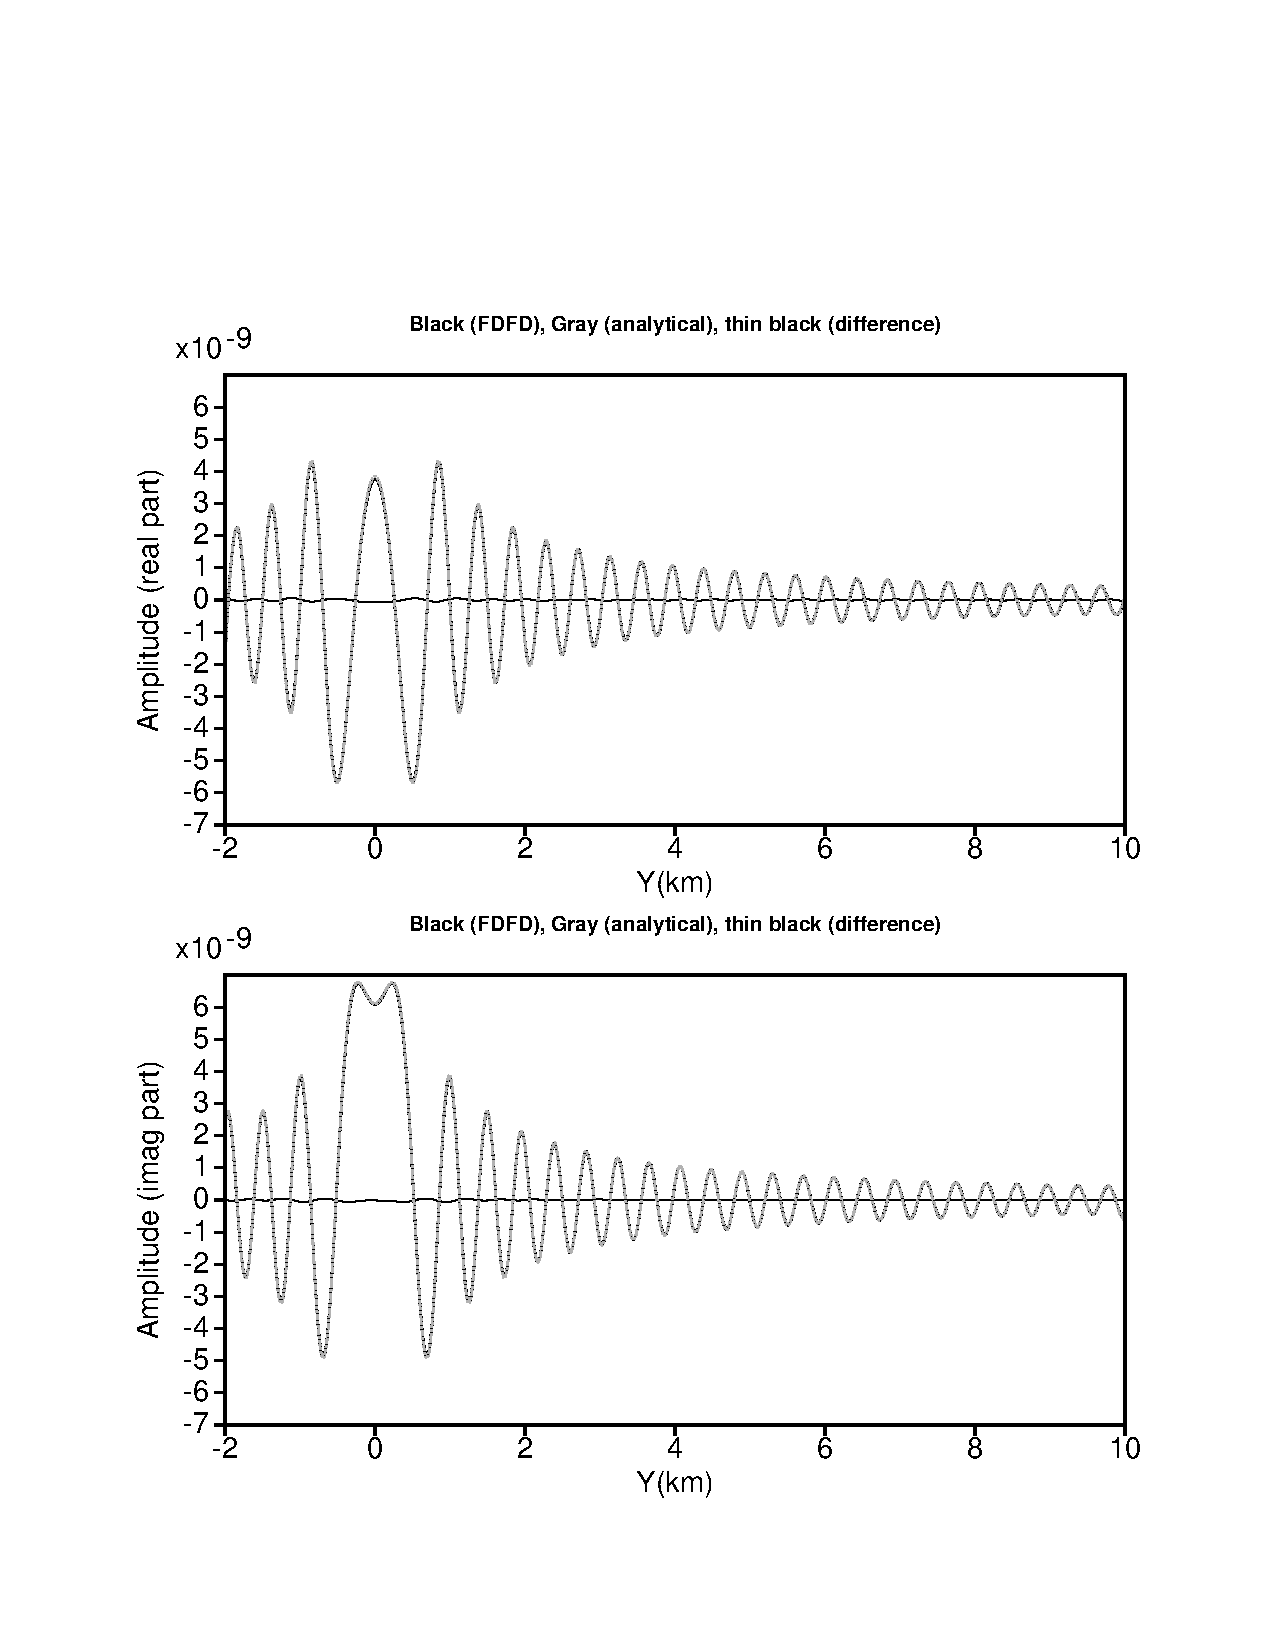
\includegraphics[width=0.7\textwidth]{images/fig_dsfdm/fig_rec_log_homogeneous_isotropic.pdf}
\caption{Homogeneous Isotropic. Infinite homogeneous isotropic medium. Validation against analytical
solution. Solution at receiver positions along the Y profile running across the shot position.}
\label{rec_log_homogeneous_isotropic} 
\end{figure}
\begin{figure}[]
\centering 
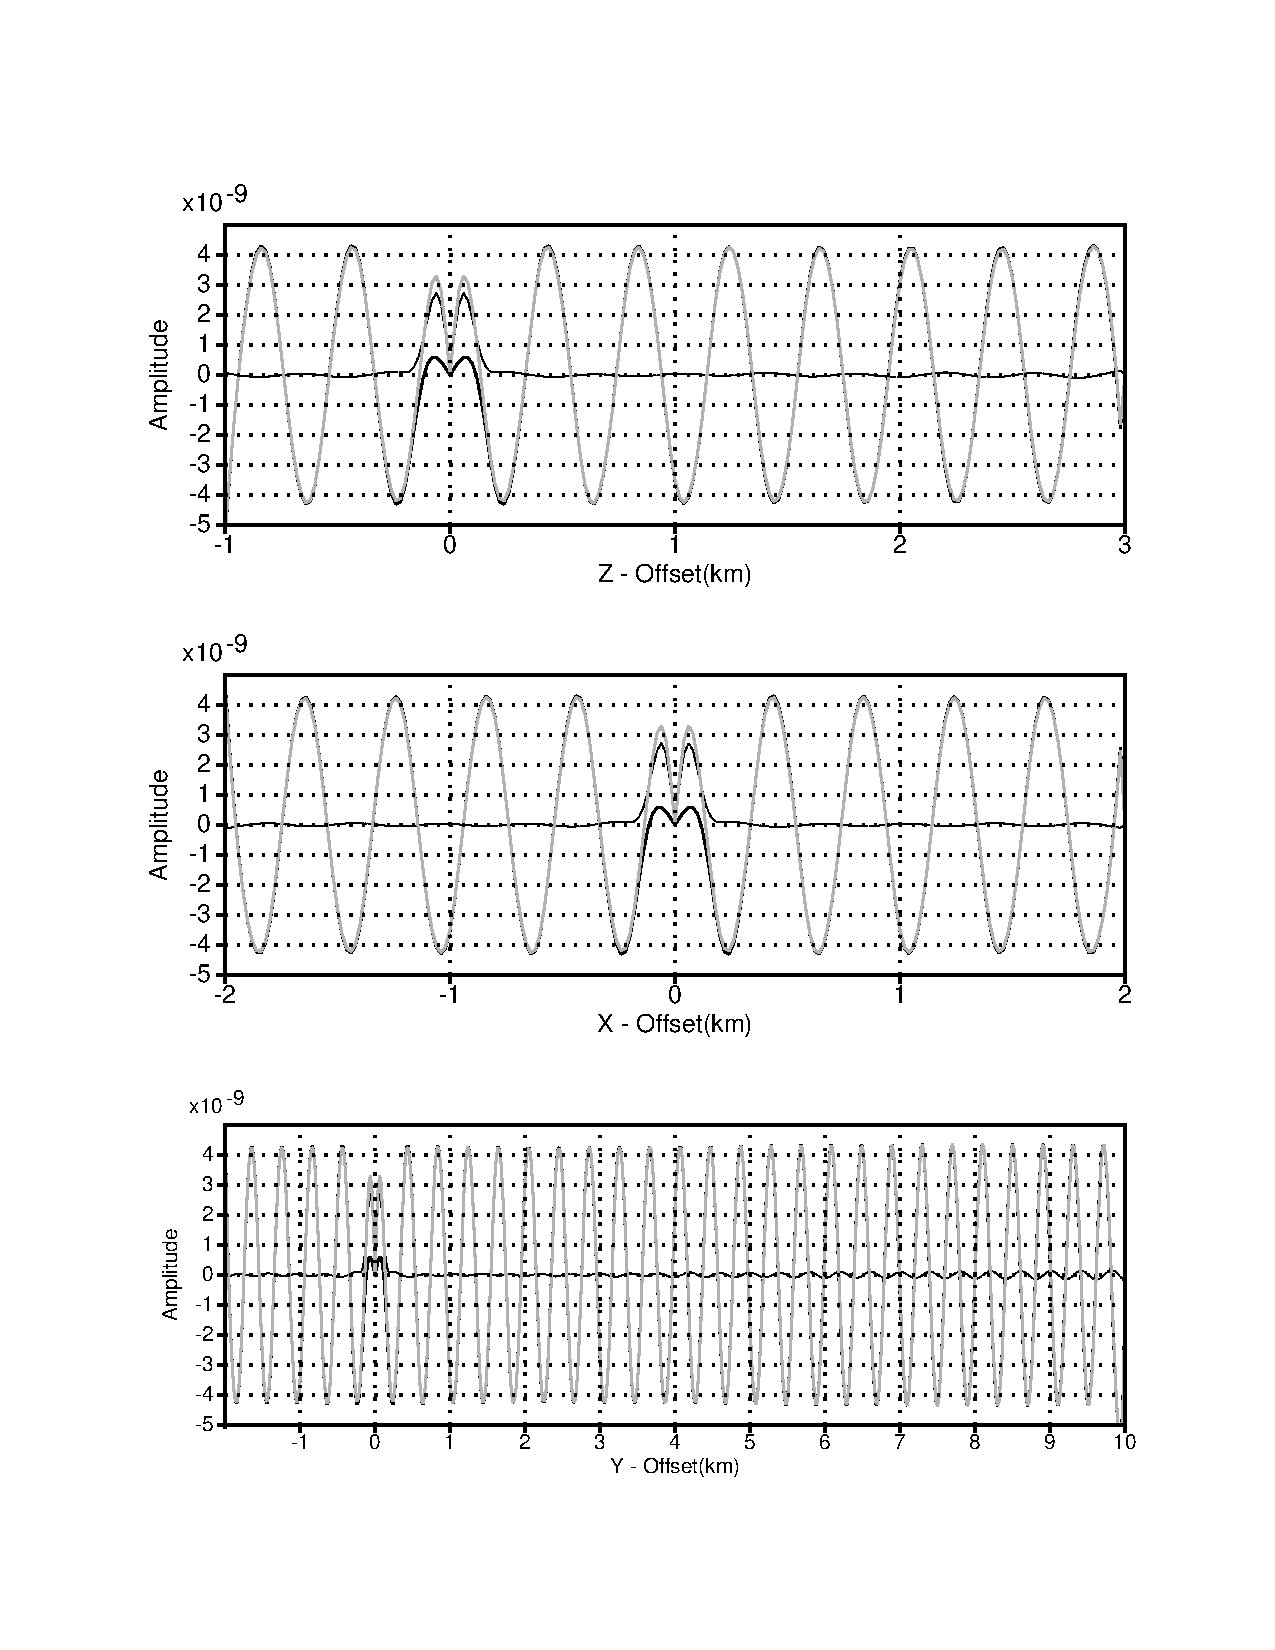
\includegraphics[width=0.7\textwidth]{images/fig_dsfdm/fig1_log_homogeneous_isotropic.pdf}
\caption{Homogeneous Isotropic. Infinite homogeneous isotropic medium. Validation against analytical
solution. Logs across shot position with correction for geometrical spreading}
\label{fig1_log_homogeneous_isotropic} 
\end{figure}
\begin{figure}[]
\centering 
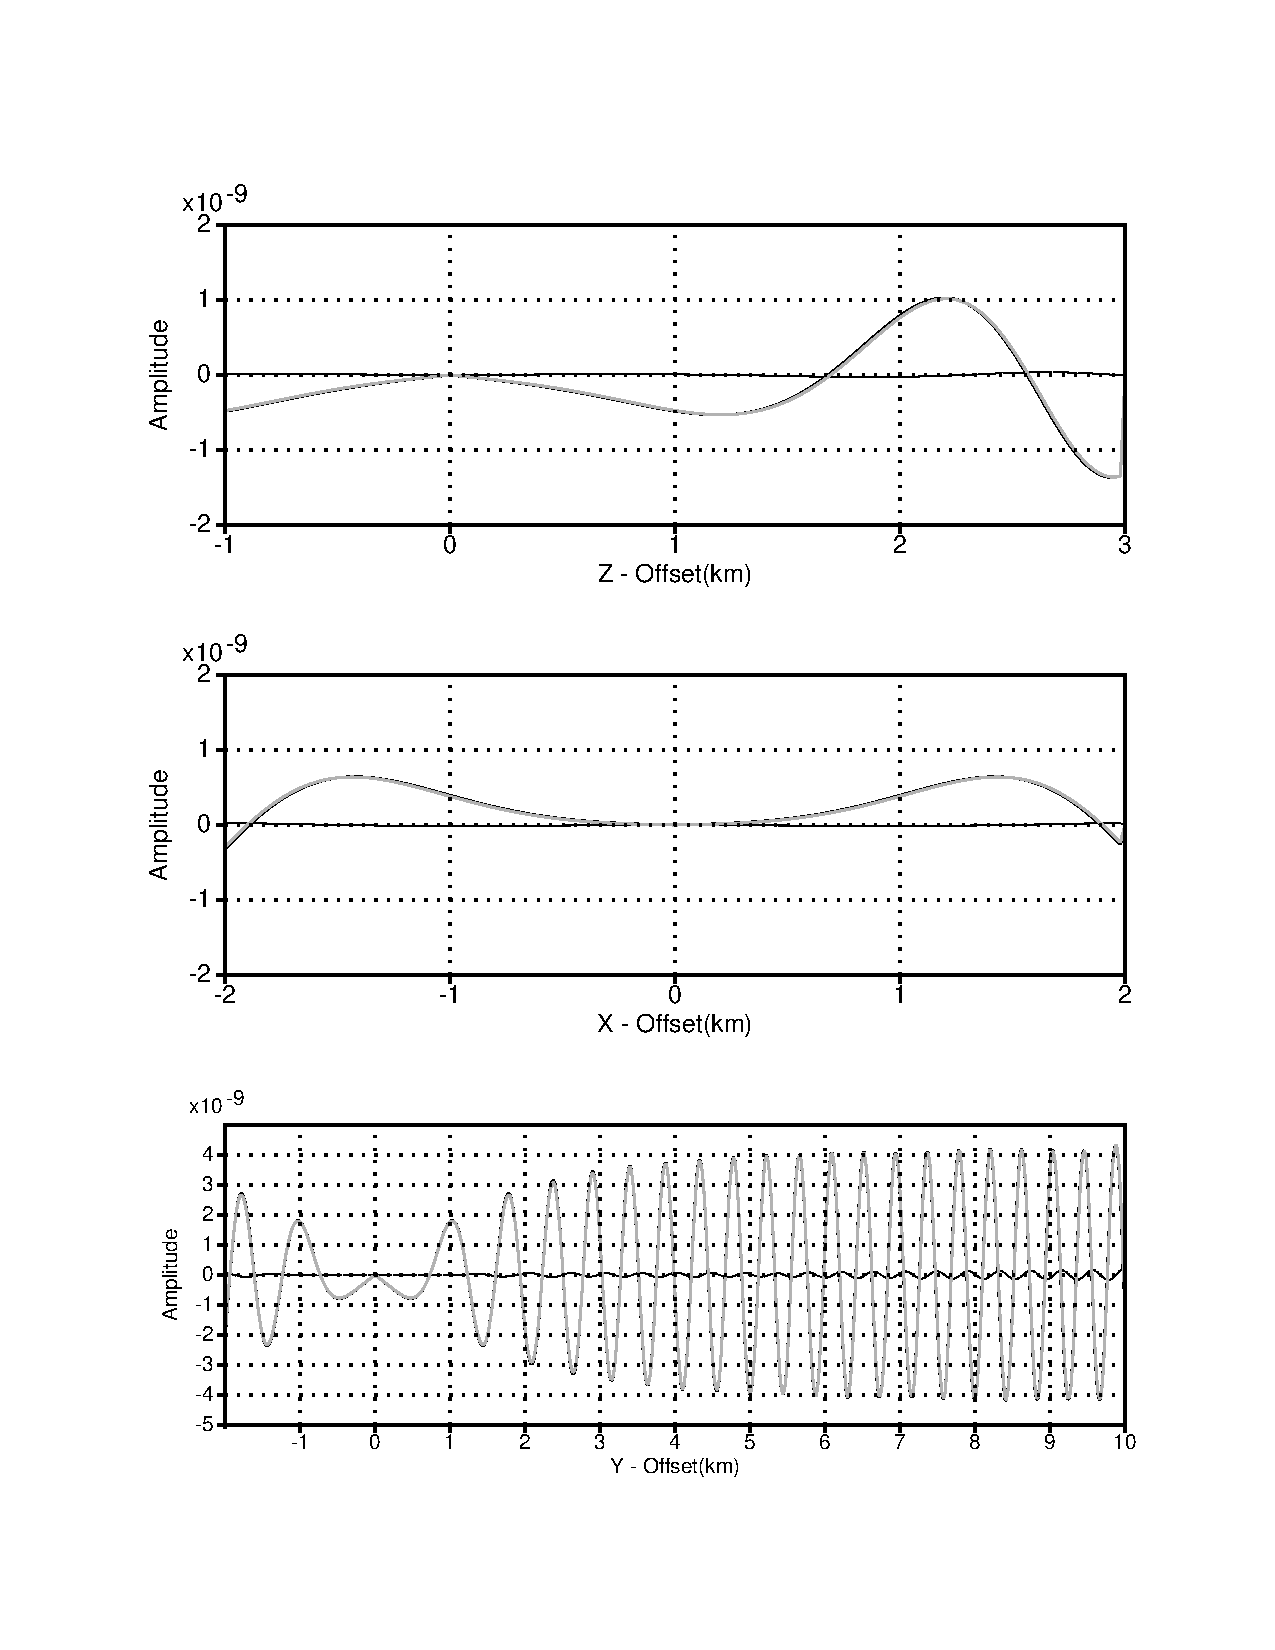
\includegraphics[width=0.7\textwidth]{images/fig_dsfdm/fig2_log_homogeneous_isotropic.pdf}
\caption{Homogeneous Isotropic. Infinite homogeneous isotropic medium. Validation against analytical
solution. Logs along the slices of Fig. ??b with correction for geometrical spreading}
\label{fig2_log_homogeneous_isotropic} 
\end{figure} 

In the following sentences, we define three test cases depending on the size of the grid to study the strong scalability of DSFDM code. This grid is a 3D dimension, $n1, n1, n1$, with PMLs. The chosen sizes of the grid are  $(n1,n2,n3)=(81,81,121)$,  $(n1,n2,n3)=(81,121,121)$ and $(n1,n2,n3)=(121,121,121)$. The grid interval is 100. We perform these tests in node cluster which contains the classical nodes and Mesca node described above. The resolution of wave propagation equation is handled by MUMPS solver. Here, we are more interested in factorization phase performing by MUMPS solver. This factorization can be doing in two ways: Full Rank and Low-Block Rank. In the following simulation, we will focus on the Full Rank option. In all the tests, we consider the number of MPI processes is always less or equal than the number of sockets (or CPU). 

The Figures \ref{TimeLU} and \ref{TimeMPIlog} show the elapsed time of the three different test cases running on classical nodes. As we can see in Figure \ref{TimeLU}, the Time of LU factorization depending on numbers of processes decreased by following a power law decay. We remark also, we obtain a good approximation when the numbers of processes is equals to a power of 2 (see Figure \ref{TimeLU2}). A log-log plot, (Figure \ref{TimeMPIlog1}), shows the strong scalability of the tests. In the case of $(n1,n2,n3)=(121,121,121)$, we observe a rapid drop of elapsed time between 2 and 8 processes and smooth descent of the curve in 8 and 16. The table \ref{fitting} shows the curve fitting of the the log scale plots (ie. $ Y= A*log(N)+B $, with N number of processes).

\begin{table}[!h]
\centering
\begin{tabular}{l|l|l}
Size & A & B  \\
 \hline
$81 \times 81 \times 121$ & -0.65 & 2.17	 \\
 $81 \times 121 \times 121$ & -0.71 & 2.5 \\
$ 121 \times 121 \times 121$ &  -0.75 & 2.86 

\end{tabular}
\caption{Parameters of the fitting curves of Elapsed time in classical nodes}
\label{fitting}
\end{table}

Similarly, we get the same remark in Mesca node (see Figure \ref{TimeMPIlog}). Here, we see a rapid growth between 2 and 4 processes different of the classical nodes. The elapsed time is fitted in log scale plot such that the slope and the intercept are given by the table \ref{fittingMesca}. For comparing the performance of Mesca and the classical nodes, we can use the execution time or the elapsed time in LU factorization. As the two architectures are different,   time may not be a good measure of comparison. We can can go further by considering the speedup that is define by Amdhal.

\begin{table}[!h]
\centering
\begin{tabular}{l|l|l}
Size & A & B  \\
 \hline
 $81 \times 81 \times 121$ & -0.62 & 2.16	\\
$81 \times 121 \times 121$ & -0.74 & 2.5 \\
$121 \times 121 \times 121$ &  -0.72 & 2.81

\end{tabular}
\caption{Parameters of the fitting curves of Elapsed time in Mesca}
\label{fittingMesca}
\end{table}



\begin{figure}
\centering 
  \begin{subfigure}[b]{0.7\textwidth}
    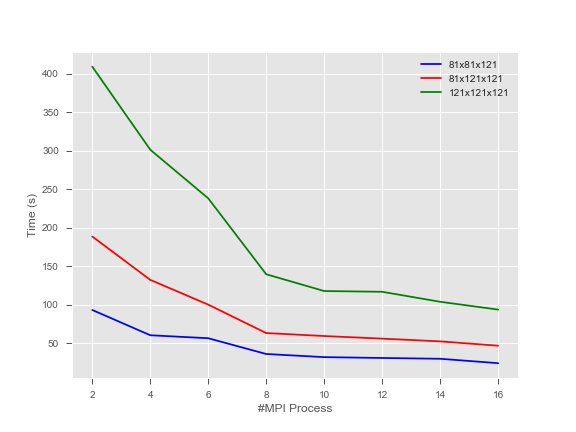
\includegraphics[width=\textwidth]{images/TimeLU.png}
    \caption{Time Elapsed for LU factorization performing in classical nodes}
    \label{TimeLU}
  \end{subfigure}
   
   \begin{subfigure}[b]{0.7\textwidth}
    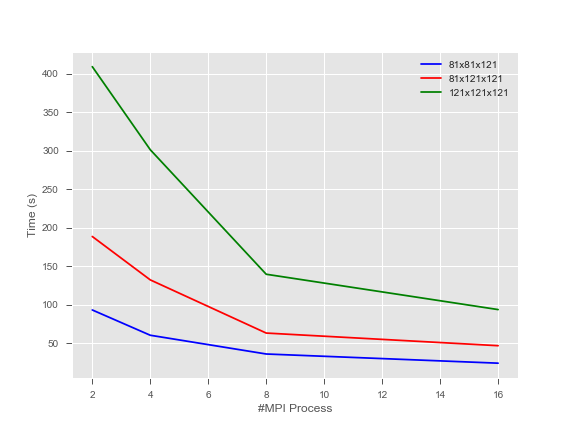
\includegraphics[width=\textwidth]{images/TimeLU2.png}
    \caption{Elapsed time for LU factorization in log scale performing in on classical nodes}
    \label{TimeLU2}
  \end{subfigure}
  
  %
  \begin{subfigure}[b]{0.7\textwidth}
    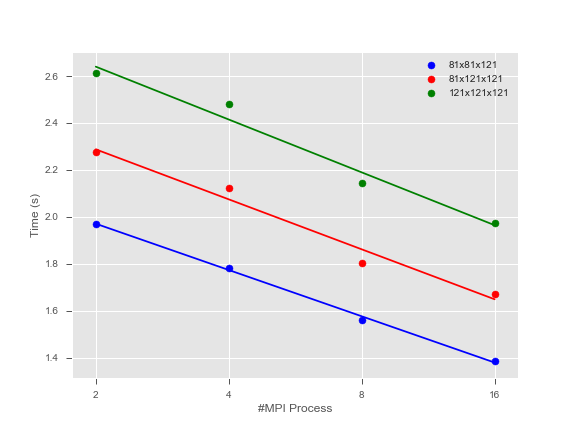
\includegraphics[width=\textwidth]{images/TimeMPIlog1.png}
    \caption{Elapsed time for LU factorization in log scale performing in on classical nodes}
    \label{TimeMPIlog}
  \end{subfigure}
  
\end{figure}
 
\begin{figure}
\centering 
  \begin{subfigure}[b]{0.7\textwidth}
    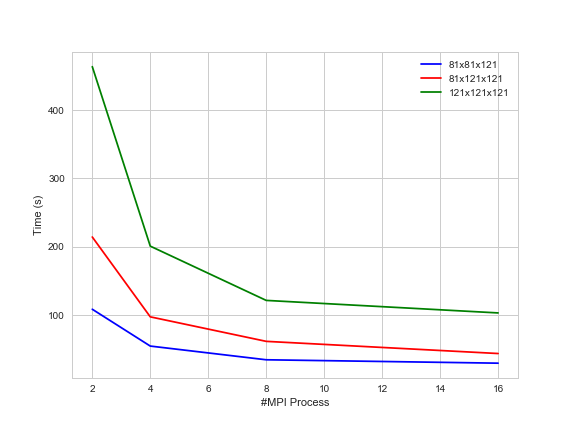
\includegraphics[width=\textwidth]{images/TimeMescaLU.png}
    \caption{Time Elapsed in LU factorization in  performing in Mesca node}
    \label{TimeMescaLU}
  \end{subfigure}
  %
  \begin{subfigure}[b]{0.7\textwidth}
    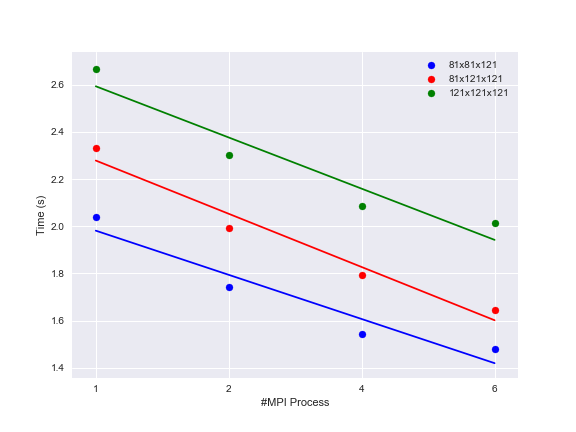
\includegraphics[width=\textwidth]{images/TimeMescaMPIlog.png}
    \caption{Elapsed time for LU factorization in log scale performing in Mesca node}
    \label{TimeMescaMPIlog}
  \end{subfigure}
\end{figure} 

\begin{figure}
\centering 
  \begin{subfigure}[b]{0.7\textwidth}
    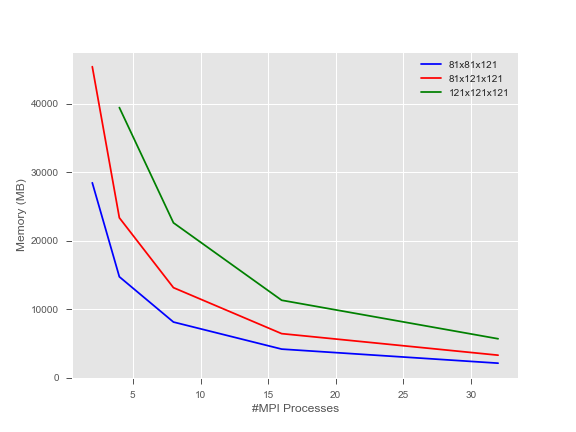
\includegraphics[width=\textwidth]{images/memoryMPI.png}
    \caption{Avg. Space in MBYTES per working proc for LU factorization on classical nodes }
    \label{memoryMPI}
  \end{subfigure}
  %
  \begin{subfigure}[b]{0.7\textwidth}
    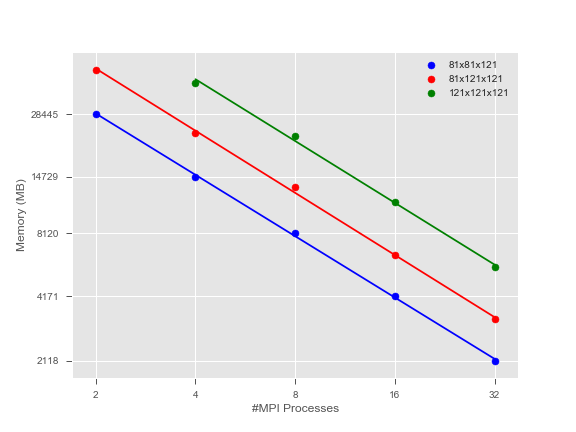
\includegraphics[width=\textwidth]{images/MemoryMPIlog.png}
    \caption{Avg. Space in MBYTES per working proc for LU factorization in log scale on classical nodes}
    \label{MemoryMPIlog}
  \end{subfigure}
\end{figure} 

\begin{figure}
\centering 
  \begin{subfigure}[b]{0.7\textwidth}
    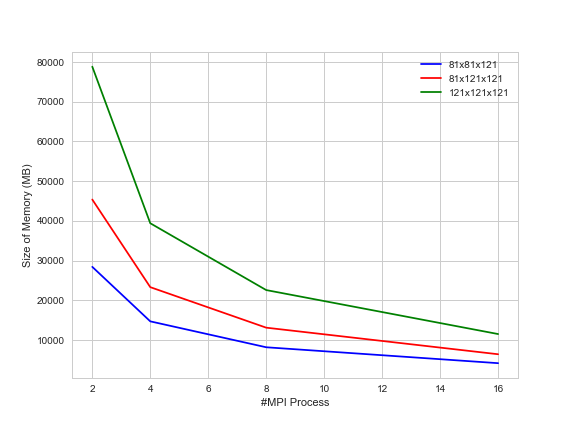
\includegraphics[width=\textwidth]{images/memoryMescaMPI.png}
    \caption{Avg. Space in MBYTES per working proc in LU factorization}
    \label{sim2}
  \end{subfigure}
  %
  \begin{subfigure}[b]{0.7\textwidth}
    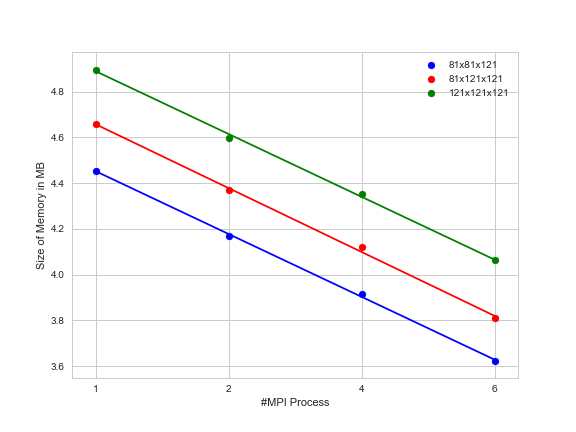
\includegraphics[width=\textwidth]{images/MemoryMescaMPIlog.png}
    \caption{Avg. Space in MBYTES per working proc in LU factorization in log scale}
    \label{sim3}
  \end{subfigure}
\end{figure} 

.............................. \newline
Comment ......................
.............................. \newline
\begin{figure}[]
\centering 
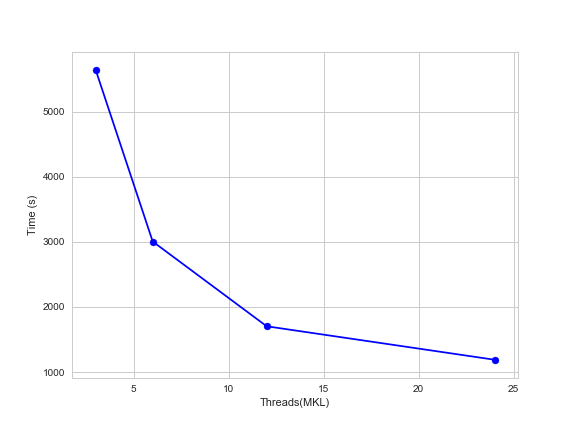
\includegraphics[width=0.75\textwidth]{images/TimeThreads.png}
\caption{Elapsed Time for LU factorization function of number of threads in Mesca node}
\label{Mesca_Time} 
\end{figure}

.............................. \newline
Comment ...................... 
.............................. \newline

\begin{figure}[]
\centering 
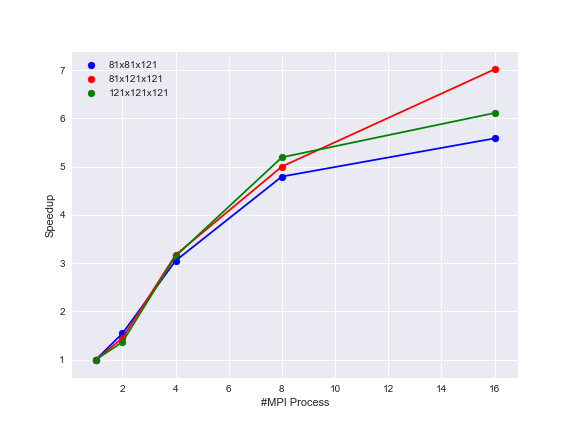
\includegraphics[width=0.75\textwidth]{images/SpeedupMesca.png}
\caption{Speedup in Mesca node}
\label{Mesca_Time} 
\end{figure}
\begin{figure}[]
\centering 
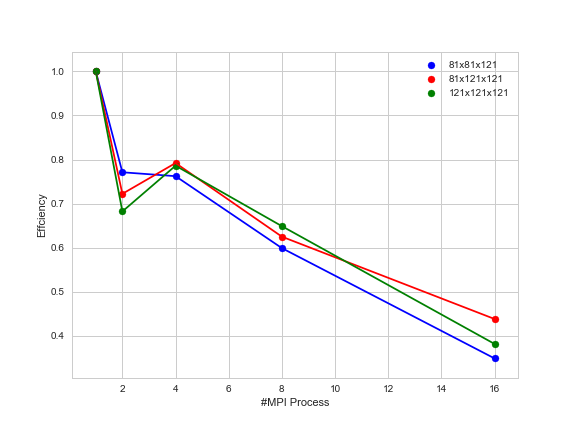
\includegraphics[width=0.75\textwidth]{images/EffciencyMesca.png}
\caption{Efficiency in Mesca node}
\label{Mesca_Time} 
\end{figure}



.............................. \newline
Comment ...................... \newline
.............................. \newline



\begin{figure}[]
\centering 
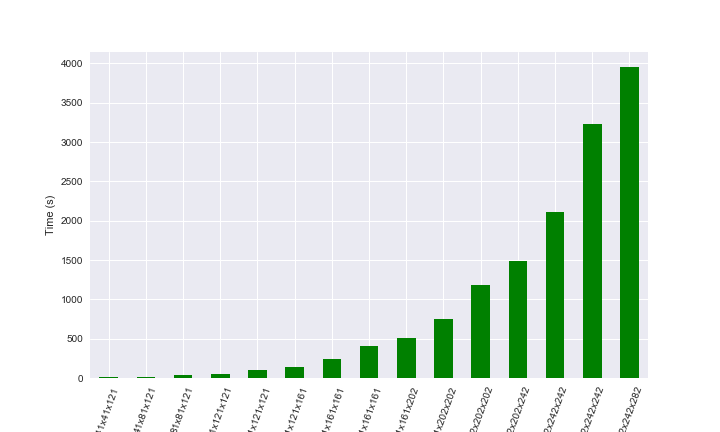
\includegraphics[width=0.75\textwidth]{images/Mesca_Time.png}
\caption{Time in LU factorization in Mesca node}
\label{Mesca_Time} 
\end{figure}
\begin{figure}[]
\centering 
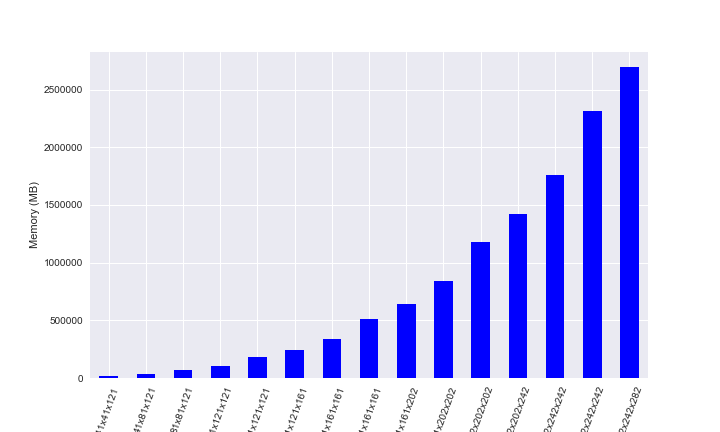
\includegraphics[width=0.75\textwidth]{images/Mesca_Memory.png}
\caption{Memory consumption in LU factorization in Mesca node}
\label{Mesca_Memory} 
\end{figure}
.............................. \newline
Comment ......................
.............................. \newline

Placement of Threads: KMP AFFINITY

\begin{table}[!h]
\centering

\label{Mesca1}
\begin{tabular}{lllllllllllll}
KMP\_AFFINITY & Grid dimensions & npml & \#MPI & \#th & \#Cores & $T_{LU}(s)$ &$Avg. Mem_{LU}/proc(MB)$ & $Mem_{LU}(MB)$ & $T(s)$ \\
 \hline
scatter &	$92 \times 181 \times 321; dz=50$ &	8 &	8 &	24 & 192 &	396.3693 & 73402 &	587218 & 7m39.295s \\
compact &	$92 \times 181 \times 321; dz=50$ &	8 & 8 &	24 & 192 &	435.1387 & 73402 &	587218 & 8m17.930s

\end{tabular}
\caption{Homogeneous Isotropic running on Mesca node}
\end{table}


.............................. \newline
Comment ......................
.............................. \newline

Case study: Ovethrust. \newline

\begin{table}[!h]
\centering

\label{amestoy}
\begin{tabular}{llllllllll}
Freq & Grid dimensions & npml &  & \#MPI & \#th & \#Cores & $T_{LU}(s)$  \\
 \hline
3.5, 4, 4.5, 5 & $ 66 \times 130 \times 230; dz=70$ & 8 & 24 & 10 & 240 & 78 \\
7 &	$ 92 \times 181 \times 321; dz=50 $ &	8 & 32 & 10	& 320 & 322 \\
10 & $ 131 \times 258 \times 458; dz=35$ &	4 &	68 & 10	& 680 &	1153

\end{tabular}
\caption{}
\end{table}

\begin{table}[!h]
\centering

\label{amestoyMesca}
\begin{tabular}{lllllllllll}
Freq & Grid dimensions & npml & \#MPI & \#th & \#Cores & $T_{LU}(s)$ & $ T(s)$ \\
 \hline
3	& $ 66 \times 130 \times 230; dz=70$ &	8 & 5 & 24	& 120 &	194.0989 & 3m42.937s  \\
3,5	& $ 66 \times 130 \times 230; dz=70$ &	8 &	8 &	15 &	120 &	98.9756 & 2m4.808s  \\
7	& $ 92 \times 181 \times 321; dz=50 $ & 8 & 8 & 20 &	160	& 439.0829 & 8m21.590s  \\
7	& $ 92\times 181 \times 321; dz=50 $ &	8 &	8 &	24 &	192	& 396.3693 & 7m39.295s	 \\							
10	& $ 131 \times 258 \times 458; dz=35$ &	4	& 8 &	24 & 192	 & 2182.6717 &	38m58.811s
\end{tabular}
\caption{}
\end{table}
\section{Profiling}
\section{Results}